\chapter{Technology}
\label{chapter-Technology}

This chapter gives an introduction to the technology stack (PHP, eZ~Publish,
eZ~Components) that is relevant to and used by the software that has been
implemented as part of this thesis.

\section{PHP}

PHP is a widely-used scripting language. Initially designed for Web
programming, it has matured to a general-purpose programming language that
supports both procedural and object-oriented programming. PHP makes strong
inroads into large-scale, business-critical Web systems. For instance,
financial institutions develop and maintain BASEL II credit and insurance
rating tools using PHP and Yahoo! runs all its business on PHP (except the core
of the search engine). As of version 5, released July 2004, the PHP language
features an object model that is similar to the ones of Java and C\# and
integrates ideas from other programming languages. The key technical
contributor to PHP's success is its sim\-pli\-city, which translates into
shorter development cycles, easier maintenance, and lower training costs. The
second one is social -- the very large and vibrant community around it, which
develops not only PHP itself but also thousands of open source applications
that can be used off-the-shelf or as references for new applications.

\cite{SB05} gives an introduction to object-oriented programming with PHP 5.

\section{eZ Publish}
\label{section-eZPublish}

eZ~Publish is the Enterprise Content Management System developed by
eZ~Systems~AS. With its framework architechture, it is both an
out-of-the-box solution as well as a platform that can be customized and
extended to suit the specific requirements of a customer.

Figure~\ref{figure-ArchitectureEZPublish3} shows an overview of the
architecture of eZ~Publish in its current version.

\begin{figure}[hbt]
\begin{center}
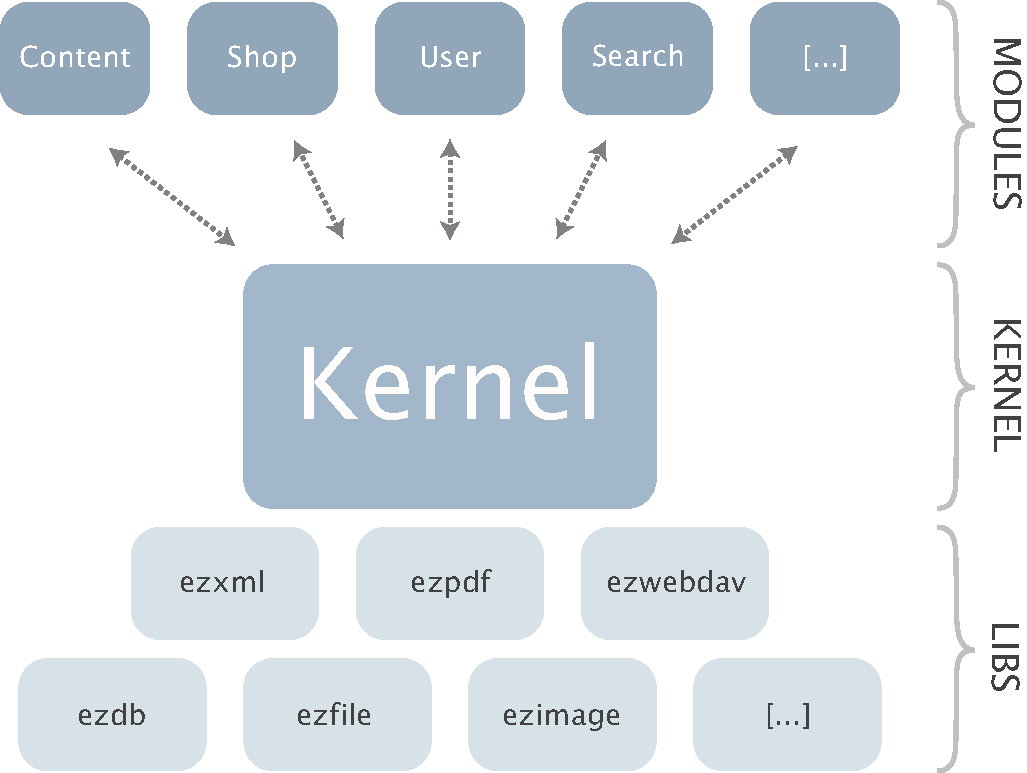
\includegraphics[width=10cm]{figures/ArchitectureEZPublish3}\\[5mm]
\end{center}
\caption{The Architecture of eZ Publish 3}
\label{figure-ArchitectureEZPublish3}
\end{figure}

The \emph{libraries} are the main building blocks of the system and are
designed as reuseable general purpose PHP classes. Although they are not
dependant on other parts of the system, some of them are not usable outside
the scope of eZ~Publish as the functionality they provide is tightly
coupled to eZ~Publish.

The \emph{kernel} makes up the system's core and is responsible, among other
things, for content handling and versioning, access control, and workflows. 

Whereas the kernel and the libraries provide rather low-level functionality,
the \emph{modules} implement the higher-level functionality of the system. They
provide web-based interfaces to functionality that is, for instance, part of
the kernel. For example, the content module provides an interface that makes
it possible to use a web browser to manage content. A module consists of two
components: at least one \emph{view} and one or more optional
\emph{fetch functions}. The former implement the actual web interface of the
module. The latter allow for the extraction of data through a module from
within a \emph{template}.

eZ~Publish uses an object-oriented approach to organize and store content
and allows for the creation of custom structures that fit the needs of the
customer. The system offers a selection of fundamental building blocks and
mechanisms that together provide a flexible content management solution. An
actual data structure is described using something called a \emph{content class}.
A content class is built up of attributes. An \emph{attribute} can be thought of
as a field, for example the ''title'' field in a structure designed to store
news articles. The description of the entire structure would be refferred to as
the ''article class''. The characteristics of an attribute inside the class are
determined by the \emph{datatype} that was chosen to represent that attribute.

\begin{figure}[hbt]
\begin{center}
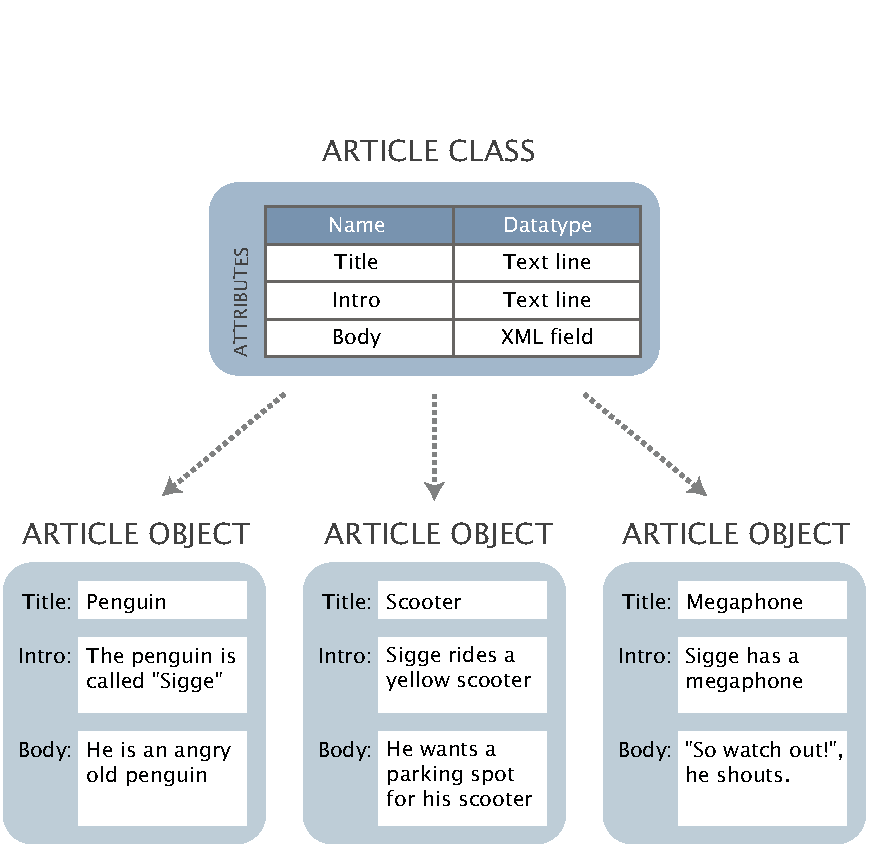
\includegraphics[width=10cm]{figures/ContentObject}\\[5mm]
\end{center}
\caption{The \emph{Content Object} abstraction of eZ Publish}
\label{figure-ContentObject}
\end{figure}

A \emph{content object} is an instance of a content class. While the class
only defines the data structure, it is the content objects themselves that
contain actual data. Once a content class is defined, several instances of
that class can be created. Figure \ref{figure-ContentObject} illustrates
this relationship of datatypes, attributes, content classes, and objects.

\section{eZ Components}
\label{section-eZComponents}

As part of the development on eZ~Publish Telemark, the next major version
of its eZ~Publish Enterprise Content Management System software, eZ~Systems~AS
has begun refactoring of core functionality from eZ~Publish itself into a
library of reusable PHP components that provide low-level functionality such
as database abstraction, object persistence and caching. This library is
called eZ~Components.

Figure \ref{figure-eZComponents} shows an overview of the eZ~Components
library. One of the design goals of the library is to minimize the number of
dependencies between its various components. A component may only depend on
the \texttt{Base} component. Optional dependencies are handled through
so-called \emph{tie-in} components that tie two components together.

\begin{figure}[hbt]
\begin{center}
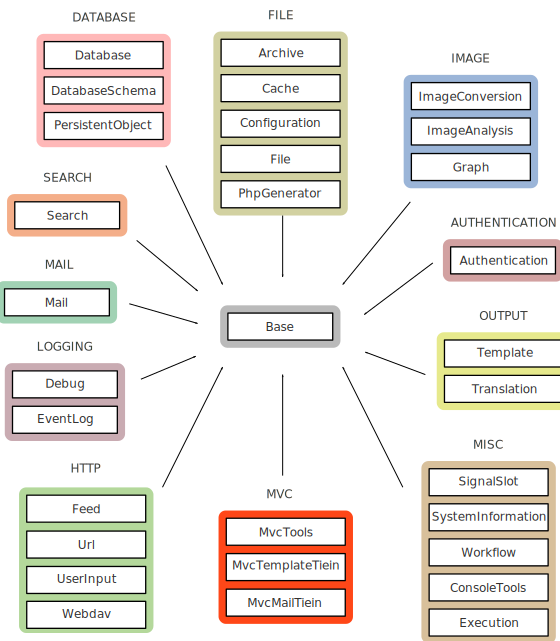
\includegraphics[width=10cm]{figures/ezcomponents}\\[5mm]
\end{center}
\caption{The eZ Components library for PHP 5.}
\label{figure-eZComponents}
\end{figure}

The workflow engine that has been developed as part of this thesis is
released under the New BSD License as part of the eZ~Components library and
utilizes the \texttt{Database} and \texttt{DatabaseSchema} components for
database abstraction and the \texttt{EventLog} component for logging
abstraction.
